\chapter{Diagramme entités-associations}

\section{Diagramme}

\begin{figure}
  \centering
  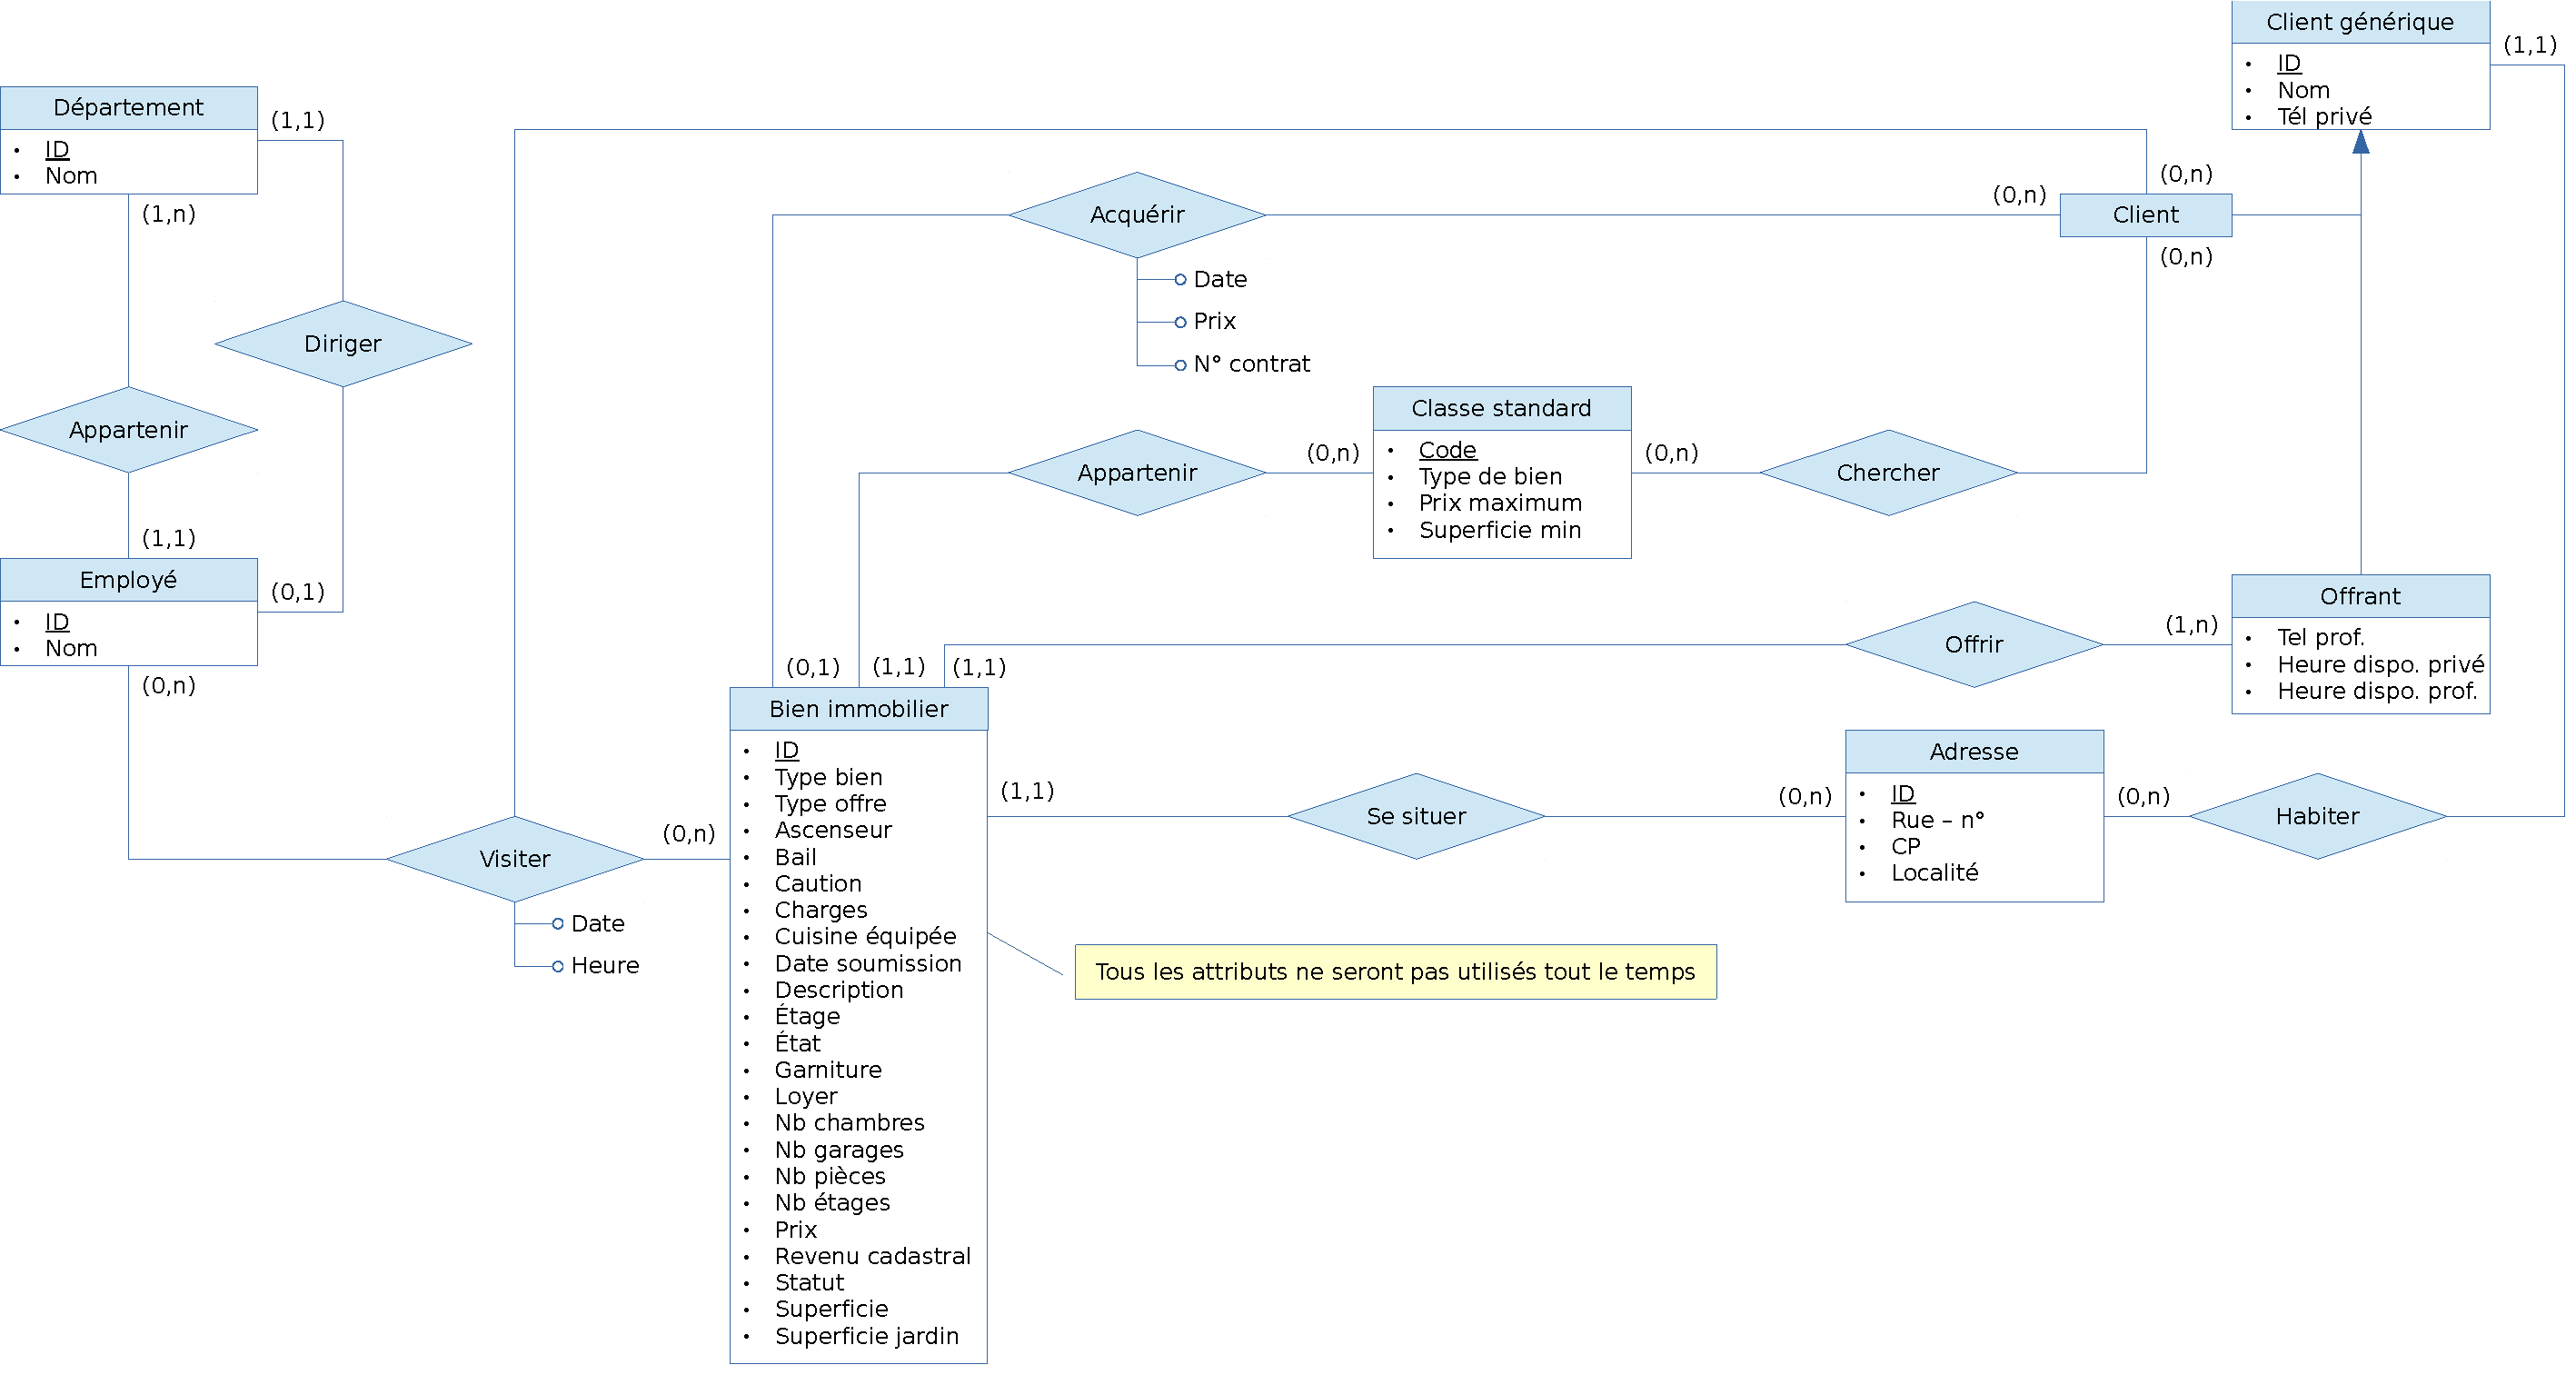
\includegraphics[angle=90,height=0.99\textheight]{IMG/er}
  \caption{Diagramme entités-associations}
  \label{img_er}
\end{figure}

La figure \refpage{img_er} illustre les entités du projet et leurs association.

\section{Rapport}

J'ai réalisé ce diagramme en deuxième lieu afin d'avoir une vue globale de l'organisation des données sur lesquelles je vais travailler.

Vu la complexité des biens immobiliers, j'ai décidé de mettre tous les attributs possibles à l'entité \og{}Bien immobilier\fg{}. Suivant la valeur des attributs \og{}Type bien\fg{} et \og{}Type offre\fg{}, les attributs auront une valeur pertinente ou non. La table \refpage{tbl_usage_attribut_bien_immobilier} nous donne les conditions de validité des attributs. Dans le tableau, un \og{}L\fg{} signifie que l'attribut est à utiliser pour une location et un \og{}V\fg{} signifie que l'attribut est à utiliser pour une vente.

\begin{table}
  \centering
  \begin{tabular}{|l|c|c|c|c|c|c|}
  \hline
  \rowcolor{gray05} \multicolumn{1}{|c|}{\textbf{Attribut}} & \multicolumn{1}{|c|}{\textbf{Studio}} & \multicolumn{1}{|c|}{\textbf{Appartement}} & \multicolumn{1}{|c|}{\textbf{Maison}} & \multicolumn{1}{|c|}{\textbf{Entrepôt}} & \multicolumn{1}{|c|}{\textbf{Emplacement}} & \multicolumn{1}{|c|}{\textbf{Terrain}} \\
  \hline
  \hline
  \textbf{Ascenseur} & L + V & L + V &  &  &  &  \\
  \hline
  \textbf{Caution} & L & L & L & L & L &  \\
  \hline
  \textbf{Charges} & L & L & L & L & L &  \\
  \hline
  \textbf{Cuisine équipée} &  & L + V & L + V &  &  &  \\
  \hline
  \textbf{Date disponible} & L + V & L + V & L + V & L + V & L + V & V \\
  \hline
  \textbf{Date soumission} & L + V & L + V & L + V & L + V & L + V & V \\
  \hline
  \textbf{Description} & L + V & L + V & L + V & L + V & L + V &  \\
  \hline
  \textbf{Étage} & L + V & L + V &  &  &  &  \\
  \hline
  \textbf{État} & V & V & V & V & V &  \\
  \hline
  \textbf{Garniture} & L & L & L & L & L &  \\
  \hline
  \textbf{Loyer} & L & L & L & L & L &  \\
  \hline
  \textbf{Nb chambres} &  & L + V & L + V &  &  &  \\
  \hline
  \textbf{Nb garages} &  & L + V & L + V &  &  &  \\
  \hline
  \textbf{Nb pièces} &  &  &  &  & L + V &  \\
 \hline
  \textbf{Nb étages} &  &  & L + V &  &  &  \\
  \hline
  \textbf{Prix} & V & V & V & V & V & V \\
  \hline
  \textbf{Revenu cadastral} & L + V & L + V & L + V & L + V & L + V & V \\
  \hline
  \textbf{Statut} & L + V & L + V & L + V & L + V & L + V & V \\
  \hline
  \textbf{Superficie} &  &  &  &  & L + V  & V \\
  \hline
  \textbf{Superficie jardin} &  & L + V & L + V &  &  &  \\
  \hline
  \textbf{Type bail} & L & L & L & L & L &  \\
  \hline
  \end{tabular}
  \caption{Utilisation des attributs de l'entité \og{}Bien immobilier\fg{}}
  \label{tbl_usage_attribut_bien_immobilier}
\end{table}

J'ai défini une entité \og{}Adresse\fg{} qui sera associée aussi bien aux clients qu'au biens immobiliers. En effet, le concept de localisation des biens immobiliers est identique à celui de localisation des clients.

J'ai défini une entité générique pour les client. Ensuite j'ai créé des entités plus spécialisées pour les clients offrants et les clients cherchant un bien. À mon sens, un client qui aujourd'hui est un client cherchant un bien peut demain être un client offrant un bien, d'où l'utilisation d'un client générique. L'entité \code{Client} n'offre actuellement pas d'attributs supplémentaires par rapport au client générique, mais bien des associations propres.